% Options for packages loaded elsewhere
\PassOptionsToPackage{unicode}{hyperref}
\PassOptionsToPackage{hyphens}{url}
\PassOptionsToPackage{dvipsnames,svgnames,x11names}{xcolor}
%
\documentclass[
  12pt,
  letterpaper,
  DIV=11,
  numbers=noendperiod]{scrartcl}

\usepackage{amsmath,amssymb}
\usepackage{iftex}
\ifPDFTeX
  \usepackage[T1]{fontenc}
  \usepackage[utf8]{inputenc}
  \usepackage{textcomp} % provide euro and other symbols
\else % if luatex or xetex
  \usepackage{unicode-math}
  \defaultfontfeatures{Scale=MatchLowercase}
  \defaultfontfeatures[\rmfamily]{Ligatures=TeX,Scale=1}
\fi
\usepackage{lmodern}
\ifPDFTeX\else  
    % xetex/luatex font selection
\fi
% Use upquote if available, for straight quotes in verbatim environments
\IfFileExists{upquote.sty}{\usepackage{upquote}}{}
\IfFileExists{microtype.sty}{% use microtype if available
  \usepackage[]{microtype}
  \UseMicrotypeSet[protrusion]{basicmath} % disable protrusion for tt fonts
}{}
\makeatletter
\@ifundefined{KOMAClassName}{% if non-KOMA class
  \IfFileExists{parskip.sty}{%
    \usepackage{parskip}
  }{% else
    \setlength{\parindent}{0pt}
    \setlength{\parskip}{6pt plus 2pt minus 1pt}}
}{% if KOMA class
  \KOMAoptions{parskip=half}}
\makeatother
\usepackage{xcolor}
\setlength{\emergencystretch}{3em} % prevent overfull lines
\setcounter{secnumdepth}{-\maxdimen} % remove section numbering
% Make \paragraph and \subparagraph free-standing
\makeatletter
\ifx\paragraph\undefined\else
  \let\oldparagraph\paragraph
  \renewcommand{\paragraph}{
    \@ifstar
      \xxxParagraphStar
      \xxxParagraphNoStar
  }
  \newcommand{\xxxParagraphStar}[1]{\oldparagraph*{#1}\mbox{}}
  \newcommand{\xxxParagraphNoStar}[1]{\oldparagraph{#1}\mbox{}}
\fi
\ifx\subparagraph\undefined\else
  \let\oldsubparagraph\subparagraph
  \renewcommand{\subparagraph}{
    \@ifstar
      \xxxSubParagraphStar
      \xxxSubParagraphNoStar
  }
  \newcommand{\xxxSubParagraphStar}[1]{\oldsubparagraph*{#1}\mbox{}}
  \newcommand{\xxxSubParagraphNoStar}[1]{\oldsubparagraph{#1}\mbox{}}
\fi
\makeatother


\providecommand{\tightlist}{%
  \setlength{\itemsep}{0pt}\setlength{\parskip}{0pt}}\usepackage{longtable,booktabs,array}
\usepackage{calc} % for calculating minipage widths
% Correct order of tables after \paragraph or \subparagraph
\usepackage{etoolbox}
\makeatletter
\patchcmd\longtable{\par}{\if@noskipsec\mbox{}\fi\par}{}{}
\makeatother
% Allow footnotes in longtable head/foot
\IfFileExists{footnotehyper.sty}{\usepackage{footnotehyper}}{\usepackage{footnote}}
\makesavenoteenv{longtable}
\usepackage{graphicx}
\makeatletter
\def\maxwidth{\ifdim\Gin@nat@width>\linewidth\linewidth\else\Gin@nat@width\fi}
\def\maxheight{\ifdim\Gin@nat@height>\textheight\textheight\else\Gin@nat@height\fi}
\makeatother
% Scale images if necessary, so that they will not overflow the page
% margins by default, and it is still possible to overwrite the defaults
% using explicit options in \includegraphics[width, height, ...]{}
\setkeys{Gin}{width=\maxwidth,height=\maxheight,keepaspectratio}
% Set default figure placement to htbp
\makeatletter
\def\fps@figure{htbp}
\makeatother

\usepackage{booktabs}
\usepackage{float}
\floatplacement{table}{H}
\usepackage{setspace}
\onehalfspacing
\usepackage{geometry}
\geometry{left=1in, right=1in, top=1in, bottom=1in}
\usepackage{lscape}
\usepackage{adjustbox}
\KOMAoption{captions}{tableheading}
\usepackage{amsmath}
\usepackage{amssymb}
\usepackage{graphicx}
\makeatletter
\@ifpackageloaded{caption}{}{\usepackage{caption}}
\AtBeginDocument{%
\ifdefined\contentsname
  \renewcommand*\contentsname{Table of contents}
\else
  \newcommand\contentsname{Table of contents}
\fi
\ifdefined\listfigurename
  \renewcommand*\listfigurename{List of Figures}
\else
  \newcommand\listfigurename{List of Figures}
\fi
\ifdefined\listtablename
  \renewcommand*\listtablename{List of Tables}
\else
  \newcommand\listtablename{List of Tables}
\fi
\ifdefined\figurename
  \renewcommand*\figurename{Figure}
\else
  \newcommand\figurename{Figure}
\fi
\ifdefined\tablename
  \renewcommand*\tablename{Table}
\else
  \newcommand\tablename{Table}
\fi
}
\@ifpackageloaded{float}{}{\usepackage{float}}
\floatstyle{ruled}
\@ifundefined{c@chapter}{\newfloat{codelisting}{h}{lop}}{\newfloat{codelisting}{h}{lop}[chapter]}
\floatname{codelisting}{Listing}
\newcommand*\listoflistings{\listof{codelisting}{List of Listings}}
\makeatother
\makeatletter
\makeatother
\makeatletter
\@ifpackageloaded{caption}{}{\usepackage{caption}}
\@ifpackageloaded{subcaption}{}{\usepackage{subcaption}}
\makeatother

\ifLuaTeX
  \usepackage{selnolig}  % disable illegal ligatures
\fi
\usepackage{bookmark}

\IfFileExists{xurl.sty}{\usepackage{xurl}}{} % add URL line breaks if available
\urlstyle{same} % disable monospaced font for URLs
\hypersetup{
  pdftitle={Analysis of Cancer Data},
  pdfauthor={Group 37: Gaoli Lin, Haowei Yan, Haotian Liu, Yizhou Gu},
  colorlinks=true,
  linkcolor={blue},
  filecolor={Maroon},
  citecolor={Blue},
  urlcolor={Blue},
  pdfcreator={LaTeX via pandoc}}


\title{Analysis of Cancer Data}
\author{Group 37: Gaoli Lin, Haowei Yan, Haotian Liu, Yizhou Gu}
\date{}

\begin{document}
\maketitle


\section{1. Introduction}\label{introduction}

Modern mass spectrometry collects thousands of molecular features, but
analyzing such high-dimensional data is challenging. Identifying key
patterns can aid early diagnosis and improve treatment. To explore the
question, the Arcene dataset will be divided into a training set and a
test set. A unique training set containing 100 samples with 5,000
randomly selected features. A fixed test set (100 samples with all
10,000 features) will be used for model evaluation. The study will
employ various classification techniques to evaluate their ability to
distinguish between cancerous and normal tissue samples. The primary
research question is whether biochemical features can accurately
differentiate between these two types of tissue. Additionally, the study
will compare different classification models, including
\textbf{Tree-based methods}, \textbf{Discriminant Analysis methods},
\textbf{SVM}, and \textbf{Neural Networks}, to identify the
best-performing model.

\section{2. Data Processing}\label{data-processing}

\subsection{2.1Initial rejection of potential
probes}\label{initial-rejection-of-potential-probes}

Based on the dataset description, we performed an initial feature
selection process to reduce the dimensionality of the data and eliminate
variables that may not provide meaningful insights for the model. We
focused on removing features with extremely low variance, as these are
typically considered to be probes or noise sequences that do not
contribute valuable information for predictive modeling. By removing
these low-variance features, we reduced the data dimensionality, which
facilitates more efficient analysis and model training, and helps to
prevent overfitting by removing redundant or irrelevant information.

\begin{figure}

\centering{

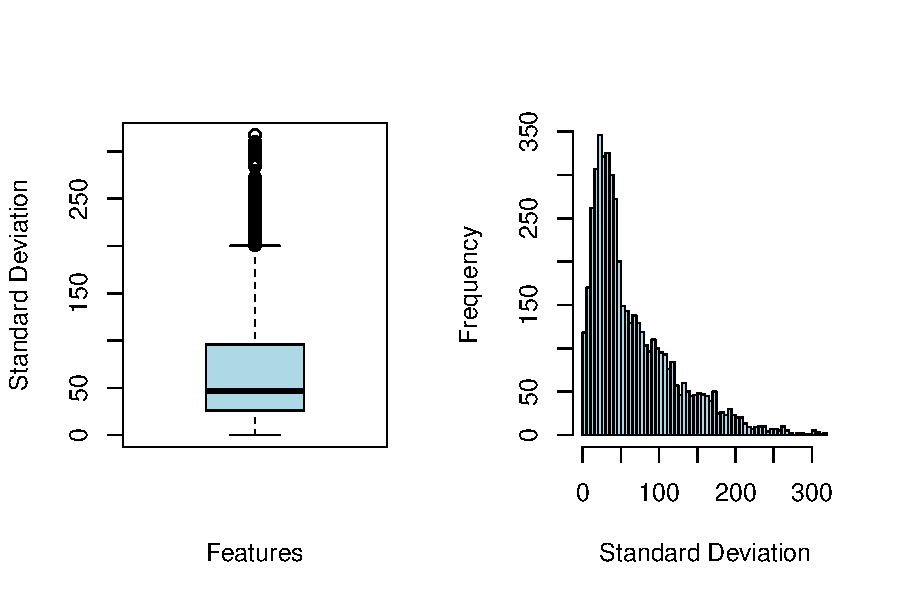
\includegraphics{me_files/figure-pdf/fig-init1-1.pdf}

}

\caption{\label{fig-init1}Variable Standard Deviation Distribution}

\end{figure}%

\subsection{2.2 Data Dimension Reduction
Processing}\label{data-dimension-reduction-processing}

PCA was further applied to reduce the dimensionality of the data. The
Kaiser criterion and the cumulative variance contribution ratio were
used to select the effective principal components. Based on these
criteria, the original dataset was updated, leading to a significant
reduction in its dimensionality. As a result, we now have three datasets
for training: the original dataset, the dataset after initial variable
selection, and the dataset after PCA dimensionality reduction. The
subsequent analysis will be conducted using each of these datasets
separately. The datasets contain features derived from different
preprocessing methods: Dataset 1: Original dataset with 5000 features.
Dataset 2: Feature selection reduced the number of features to 1824.
Dataset 3: Principal Component Analysis (PCA) reduced the feature count
to 47.

\section{3. Formal data analysis}\label{formal-data-analysis}

\subsection{3.1 Discriminant-based
methods}\label{discriminant-based-methods}

\subsubsection{3.1.1 Linear Discriminant
Analysis}\label{linear-discriminant-analysis}

LDA is a classification method based on probability distributions. It
assumes that all classes share the same covariance structure, resulting
in a linear decision boundary. This assumption makes LDA effective when
the class distributions are similar but may limit its performance when
dealing with more complex data.

However, LDA relies on the assumption of homogeneous covariance matrices
across classes.The Box's M-test for homogeneity of covariance matrices
produced a very small p-value, suggesting that the assumption of equal
covariance matrices does not hold. The violation of this assumption
suggests that LDA may not be the most suitable method for this dataset,
as it could lead to suboptimal classification performance.

\subsubsection{3.1.2 Quadratic Discriminant
Analysis}\label{quadratic-discriminant-analysis}

QDA extends LDA by allowing each class to have its own covariance
structure, leading to more flexible, curved decision boundaries. This
flexibility makes QDA suitable for non-linearly separable data, but it
also increases the risk of overfitting, especially when the dataset is
small.

Two classification models, LDA and QDA, were applied to the data. The
accuracy of LDA was 73\%, with a confusion matrix showing 45 true
negatives, 28 true positives, 11 false positives, and 16 false
negatives. QDA achieved a higher accuracy of 79\%, with 48 true
negatives, 31 true positives, 8 false positives, and 13 false negatives.
The ROC curves for both models were plotted, and the AUC values were
displayed. QDA had a higher AUC than LDA, indicating better performance
in distinguishing between the two classes.

\begin{figure}[H]

{\centering 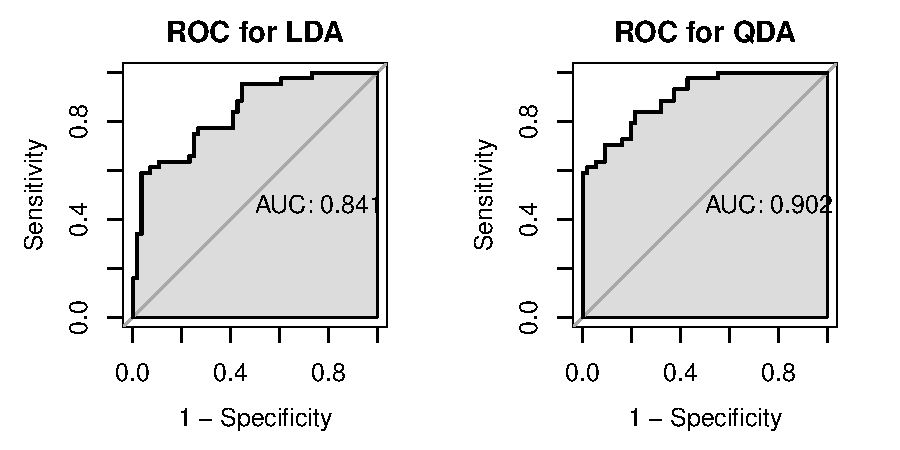
\includegraphics{me_files/figure-pdf/ROC of LDA and QDA-1.pdf}

}

\caption{ROC}

\end{figure}%

\subsection{3.2 Tree-based methods}\label{tree-based-methods}

\subsubsection{3.2.1 Classification Tree}\label{classification-tree}

Classification Tree partition the feature space into a number of
disjoint and non-overlapping regions.And predict the class of a given
observation as the most commonly occurring class of training
observations is the region to which it belongs. A classification tree is
typically suitable for smaller datasets because it is easy to interpret
during the training process and can quickly generate predictions. The
analysis was then performed using the dataset processed with PCA

\begin{figure}

\centering{

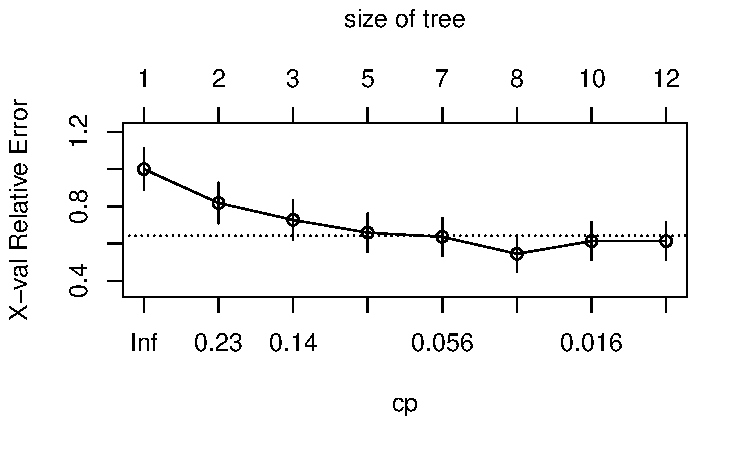
\includegraphics{me_files/figure-pdf/fig-tree1-1.pdf}

}

\caption{\label{fig-tree1}Model Performence with CP}

\end{figure}%

The pruning process is based on the complexity parameter (cp) selection.
The optimal cp is chosen as the largest value within the range where the
cross-validation error remains within one standard deviation of the
minimum error.Based on this criterion, a cp of 0.032 is selected to
prune the new tree.

\begin{figure}

\centering{

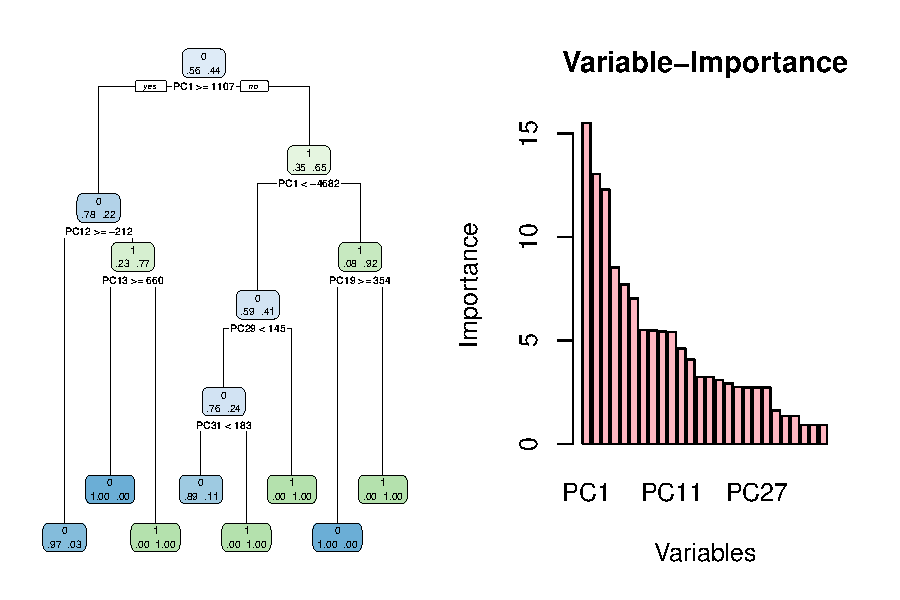
\includegraphics{me_files/figure-pdf/fig-tree2-1.pdf}

}

\caption{\label{fig-tree2}Pruned Classification Tree (cp=0.032)}

\end{figure}%

The classification tree also highlights the importance of variables,
showing that PC1 is the most significant, followed by PC12 and PC2.
Variables like PC18, PC13, PC21, and PC24 are considered less important.

The test accuracy is 0.68, indicating poor performance. While the
classification tree has some predictive ability, its overall
effectiveness is limited.

\subsubsection{3.2.2 Bagging Tree}\label{bagging-tree}

Bagging involves repeatedly drawing samples from the original dataset
and building a classification tree on each bootstrapped sample. For each
test observation, the class predicted by each tree is recorded. The
final prediction is determined by a majority vote, where the most
frequent class across all predictions is chosen. To find the minimum
number of trees that stabilize the OOB error, the model was trained with
varying tree numbers, and the OOB error was monitored. Once the error
stabilized, the smallest number of trees achieving this was selected to
build the final Bagging Tree model.

Since bagging is an ensemble method that uses multiple classification
trees, it typically requires more data to effectively train the trees
and improve prediction accuracy through ensemble learning. Therefore,
using a larger dataset (the dataset after initial variable selection)
allows better utilization of the data's diversity, enhancing the model's
stability and generalization ability.

\begin{figure}

\centering{

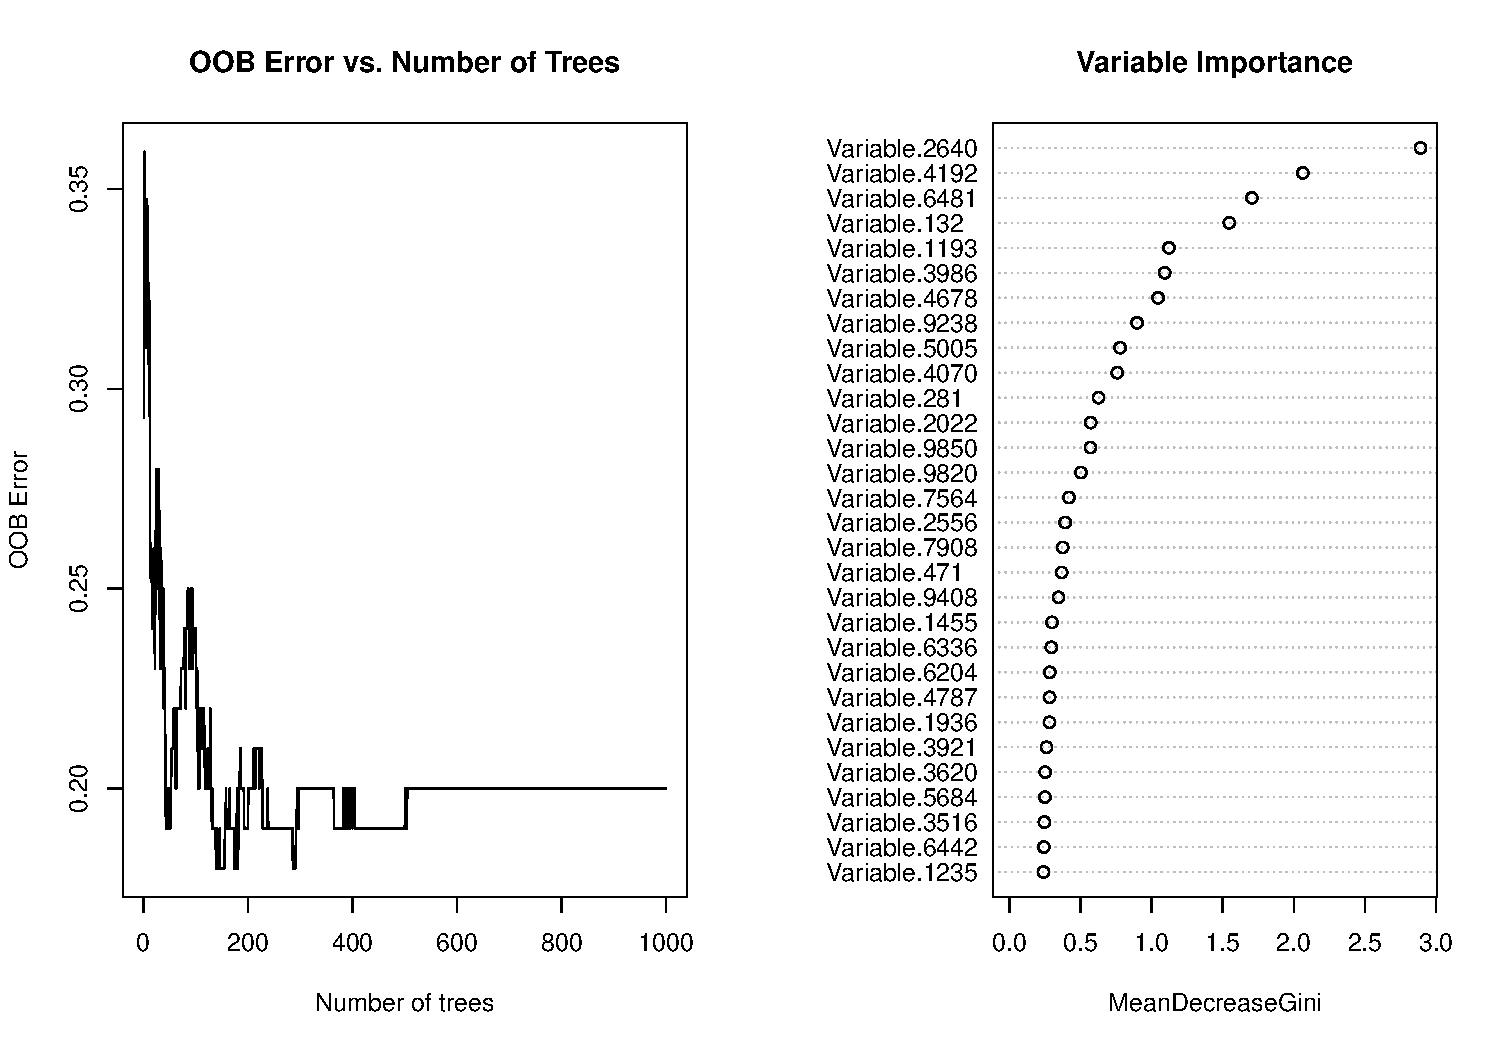
\includegraphics{me_files/figure-pdf/fig-tree5-1.pdf}

}

\caption{\label{fig-tree5}Model Performance}

\end{figure}%

According to the Bagging Tree, Variable.2640 is the most important
factor, followed by Variable.4192 and Variable.6481, Variable.132 and
Variable.1193, Variable.6442 and Variable.1235 are relatively
unimportant.The Accuracy of test is 0.79, which is good. Showing the
Bagging Tree has good classification ability.

\subsubsection{3.2.3 Random Forests}\label{random-forests}

Random forests improve upon Bagging Trees by reducing the correlation
between individual trees. By randomly excluding a subset of variables at
each split, the trees become more diverse, leading to more stable and
reliable predictions. Similarly, the model was trained using the dataset
after initial variable selection.

\begin{figure}

\centering{

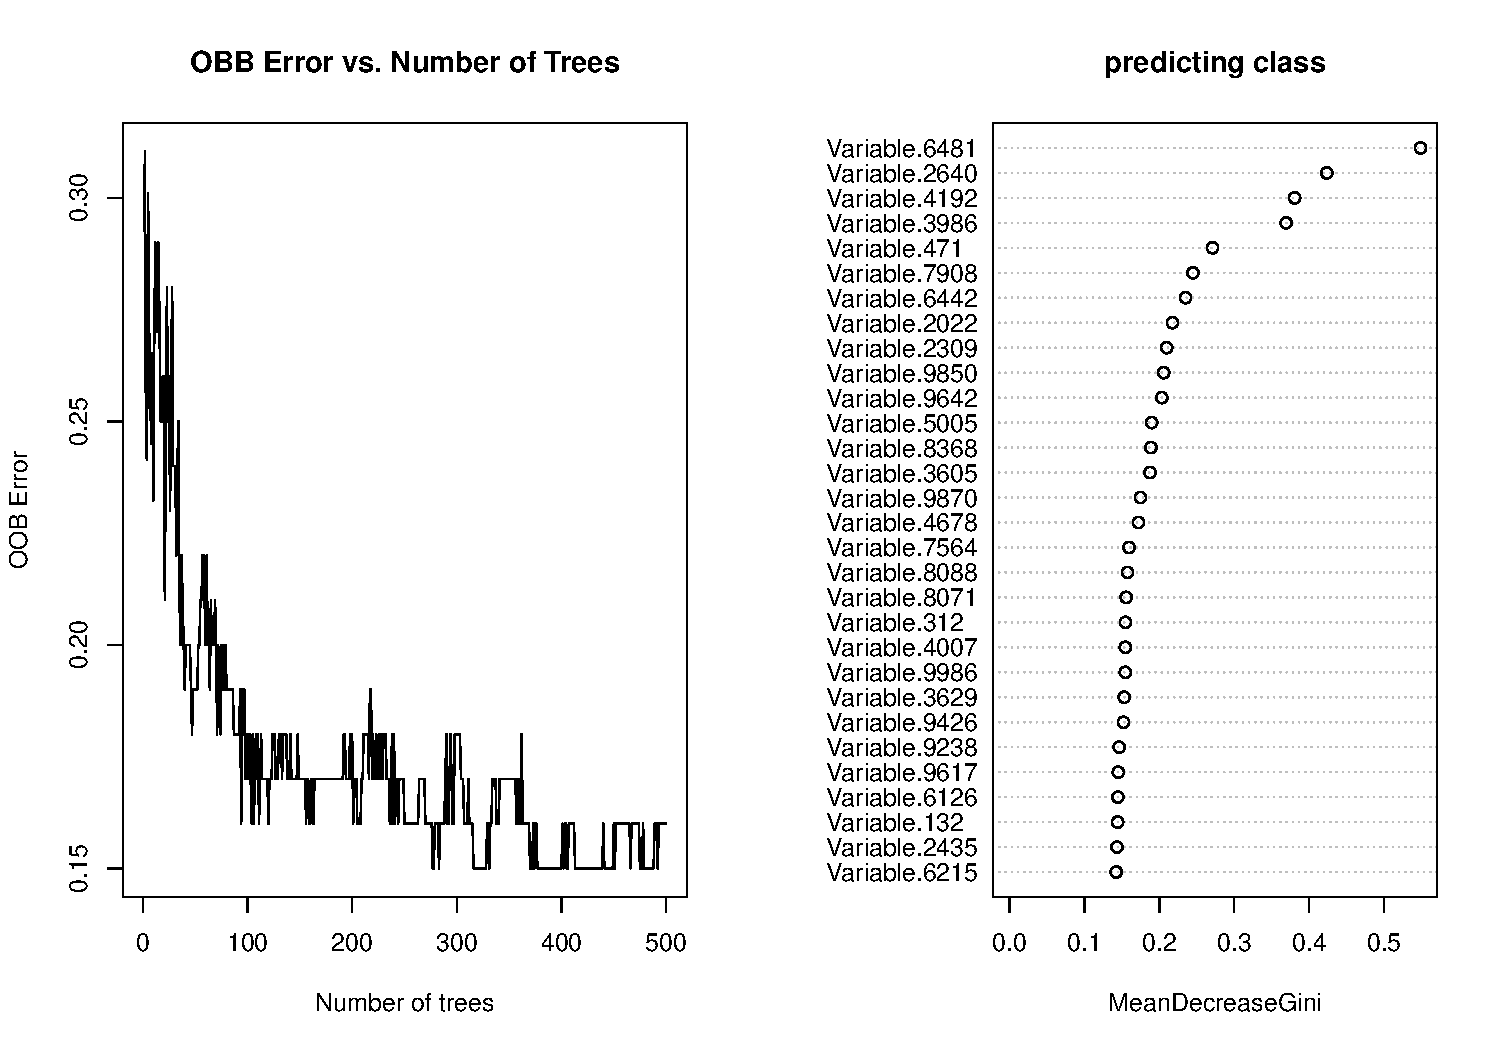
\includegraphics{me_files/figure-pdf/fig-tree8-1.pdf}

}

\caption{\label{fig-tree8}Model Performance}

\end{figure}%

According to the random forests, Variable.2640 and Variable.4192, which
were also important in the Bagging model, remain influential.

\begin{figure}

\centering{

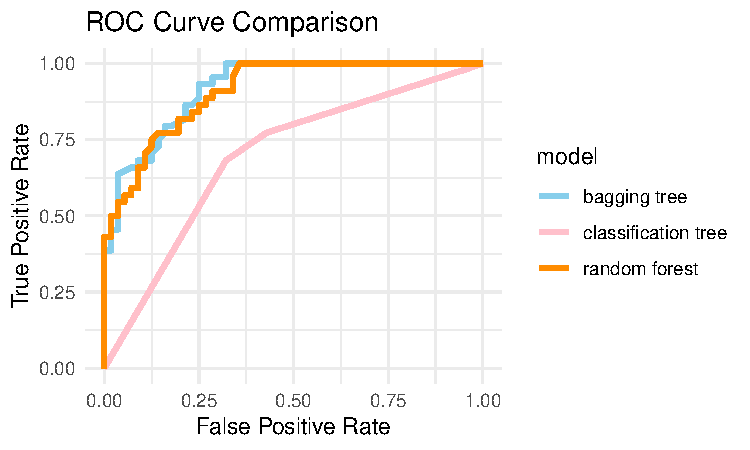
\includegraphics{me_files/figure-pdf/fig-tree10-1.pdf}

}

\caption{\label{fig-tree10}ROC Plot Compare}

\end{figure}%

The ROC comparison shows that the AUC values for the classification
tree, bagging tree, and random forest are 0.6936, 0.8953, and 0.9111,
respectively.Since the random forest achieves the highest AUC, it
demonstrates the best predictive performance among the three models.

\subsection{3.3 SVM}\label{svm}

Support Vector Machine (SVM) is a classification algorithm that finds
the optimal boundary between different classes by maximizing the margin
between data points. It identifies key data points, known as support
vectors, that are closest to the decision boundary and uses them to
define the classification rule. SVM is effective for high-dimensional
datasets and works well with small to medium-sized data. So for each
dataset, SVM models were trained, tested, and optimized identify the
best hyperparameters.

For Dataset 1, a linear kernel was optimal, while for Datasets 2 and 3,
an RBF kernel performed better. Feature selection dataset(1800 features)
provided the best performance in accuracy and AUC, while PCA dataset(40
features) caused a slight accuracy drop but remains a viable
dimensionality reduction method.

\begin{longtable}[]{@{}llll@{}}
\toprule\noalign{}
Dataset & Features & Accuracy & AUC \\
\midrule\noalign{}
\endhead
\bottomrule\noalign{}
\endlastfoot
Original & 5000 & 0.84 & 0.930 \\
Feature selection & 1824 & 0.88 & 0.948 \\
PCA Reduction & 47 & 0.81 & 0.924 \\
\end{longtable}

\begin{center}
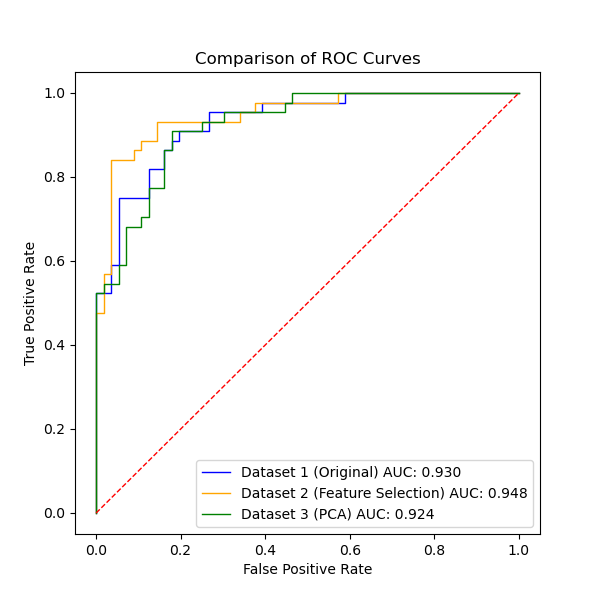
\includegraphics[width=4in,height=4in]{svm.png}
\end{center}
\#\# 3.4 Neural networks Neural networks enhance predictive performance
by capturing complex nonlinear relationships between features and the
target variable. With multiple hidden layers and structured activation
functions, they learn intricate patterns in the data and reduce
dependence on any single feature, improving generalization. To save
computational resources and retain as much information as possible, the
model was trained using the dataset after initial variable selection and
the dataset after PCA process.

\subsubsection{3.4.1 Simple Neural
networks}\label{simple-neural-networks}

A simple neural network was designed with one hidden layer based on the
dataset after the PCA process. This choice was made because the
dimensionality of the data after PCA is smaller, and a simpler network
structure is sufficient to capture the necessary information.

The model's performance was satisfactory, with an accuracy of 0.73 and
an AUC of 0.76. However, there is still room for improvement in the
neural network to enhance its performance further.

\subsubsection{3.4.2 Multilayer Neural
Network}\label{multilayer-neural-network}

To enhance the model's learning capacity, we increased the number of
neurons in the first hidden layer to 533, improving its ability to
capture important features. In the subsequent hidden layers, we
progressively reduced the number of neurons to 256, 60, and finally 20,
in order to refine the model's representation and reduce the risk of
overfitting. This layered architecture allows the network to extract
high-dimensional features in the initial layers and gradually distill
the most relevant information in the deeper layers. The model was
trained using the dataset after initial variable selection, which
provided more informative input for learning.

The training performance improved significantly, with the AUC increasing
from 0.64 to 0.95. This dramatic improvement suggests that the adjusted
network architecture effectively enhanced the model's ability to learn
complex patterns, leading to a much better classification performance.
The increased network capacity in the initial layers allowed for better
feature extraction, while the gradual reduction in neurons helped refine
the representations, ultimately resulting in a more robust and
well-generalized model.

\begin{figure}[H]

{\centering 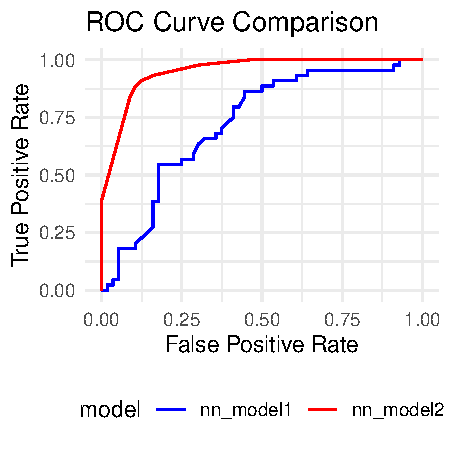
\includegraphics{me_files/figure-pdf/nnROC-1.pdf}

}

\caption{ROC of nn1 and nn2}

\end{figure}%

\section{4. Conclusion:}\label{conclusion}

Based on the results, the neural network model performed the best, with
an accuracy of 0.89 and an AUC of 0.950, closely followed by the support
vector machine (SVM) with an accuracy of 0.88 and AUC of 0.948. Among
the tree-based models, random forests achieved the highest AUC (0.911)
and accuracy (0.81), outperforming both bagging trees and classification
trees. The linear discriminant analysis (LQA) and quadratic discriminant
analysis (QDA) models showed comparable performance with accuracies of
0.73 and 0.79, and AUC values of 0.908 and 0.902, respectively. Overall,
the results indicate that more complex models, particularly neural
networks and SVM, offer the best predictive performance.

\begin{longtable}[]{@{}lll@{}}
\toprule\noalign{}
Classification Model & Accuracy & AUC \\
\midrule\noalign{}
\endhead
\bottomrule\noalign{}
\endlastfoot
Classification tree & 0.68 & 0.693 \\
Bagging tree & 0.79 & 0.895 \\
Random forests & 0.81 & 0.911 \\
LQA & 0.73 & 0.908 \\
QDA & 0.79 & 0.902 \\
SVM & 0.88 & 0.948 \\
Neural networks & 0.89 & 0.950 \\
\end{longtable}




\end{document}
